%&latexf
\documentclass{kclthesis}
\usepackage{color}
\usepackage[nottoc,notlot,notlof]{tocbibind}
\usepackage{hyperref}
\usepackage{verbatim}
\usepackage{stmaryrd}
\usepackage{fancyhdr}
\usepackage{subfigure}

% nomenclature 
%\usepackage[intoc]{nomencl}
% glossaries
\usepackage[toc, acronym]{glossaries} 

\linespread{1.5}
\newfam\msbfam
\def\Bbb#1{\fam\msbfam\relax#1}

\newtheorem{theorem}{Theorem}[section]
\newtheorem{exa}{Example}[section]
\newtheorem{corollary}[theorem]{Corollary}
\newtheorem{lemma}[theorem]{Lemma}
\newtheorem{proposition}[theorem]{Proposition}

\theoremstyle{definition}
\newtheorem{definition}[theorem]{Definition}
\newtheorem{remark}[theorem]{Remark}
\newtheorem{notation}[theorem]{Notation}
\newtheorem{assumption}[theorem]{Assumption}
\newtheorem{conjecture}[theorem]{Conjecture}

\newcommand{\ind}{1\hspace{-2.1mm}{1}} %Indicator Function
\newcommand{\I}{\mathtt{i}}
\newcommand{\D}{\mathrm{d}}
\newcommand{\E}{\mathrm{e}}
\newcommand{\RR}{\mathbb{R}}
\newcommand{\sgn}{\mathrm{sgn}}
\newcommand{\atanh}{\mathrm{arctanh}}
\def\equalDistrib{\,{\buildrel \Delta \over =}\,}
\numberwithin{equation}{section}
\def\blue#1{\textcolor{blue}{#1}}
\def\red#1{\textcolor{red}{#1}}

% customize
\title{Super duper test title - A Better approach}
\author{John Doe}
\modulecode{7CCSMPRJ}
\submissiontitle{Individual Project Submission 2015/16}
\studentnumber{XXXXX}
\programme{MSc Web Intelligence MSc}
\supervisor{Dr Frankenstein}
%\wordcount{XXXXXXX}


\usepackage{draftwatermark}
\SetWatermarkText{DRAFT}
\SetWatermarkScale{8}



%\makenomenclature
\makeglossaries




\begin{document}
\pagenumbering{gobble}


%%%%%% depends what you like, might try out the other frontpage as well
\maketitle 		% official styled layout
\maketitleTwo 	% adapted layout which looks nicer from my point of view.

%%%%%% empty page after main page.
\newpage
\thispagestyle{empty}
\mbox{}
\newpage
%%%%%% Abstract
\section*{Abstract}
Lorem ipsum dolor sit amet, consetetur sadipscing elitr, sed diam nonumy eirmod tempor invidunt ut labore et dolore magna aliquyam erat, sed diam voluptua. At vero eos et accusam et justo duo dolores et ea rebum. Stet clita kasd gubergren, no sea takimata sanctus est Lorem ipsum dolor sit amet. Lorem ipsum dolor sit amet, consetetur sadipscing elitr, sed diam nonumy eirmod tempor invidunt ut labore et dolore magna aliquyam erat, sed diam voluptua. At vero eos et accusam et justo duo dolores et ea rebum. Stet clita kasd gubergren, no sea takimata sanctus est Lorem ipsum dolor sit amet. 
%%%%%% Table of contents

\pagenumbering{roman}
\setcounter{tocdepth}{4}
\tableofcontents
\newpage
%%%%%%%%%%%%%%%%%%%%%%%%%%%%%%%%%%%%%%%%%%%%%%%%%%%%
\thispagestyle{empty}
 
\listoffigures
 
\listoftables
 
\newpage
\mbox{}\newline\vspace{10mm} \mbox{}\LARGE
%
{\bf Acknowledgements} \normalsize \vspace{5mm}

I would like to thank my supervisor.....

\fancyhead{}
\fancyfoot{}
\pagestyle{fancy} 
%\fancyhead{\sffamily\small \thepage}
%\fancyhead{\sffamily\small \nouppercase{\rightmark}}
\fancyhead[RO,LE]{\sffamily\small \thepage}
\fancyhead[LO,RE]{\sffamily\small \nouppercase{\rightmark}}
\renewcommand{\headrulewidth}{0.4pt}
\renewcommand{\footrulewidth}{0.0pt}
%%%%%%%%%%%%%%%%%%%%%%%%%%%%%%%%%%%%%%%%%%%%%%%%%%%%

%%%%%% Main content
\pagenumbering{arabic}
\section{Introduction}
\subsection{Project Aims, Objectives and Introduction} 
It gives a basic background of the work.  The problems and project objectives should be clearly stated.  The techniques and approaches used to deal with the problem should be stated with reasons, and the contributions and main results achieved should be stated clearly.  The structure of the report can be described briefly at the end see \autoref{sub:background}.
\subsection{Background and Literature Survey} \label{sub:background}
 It gives an overall picture about the work with a clear review of the relevant literature.  The background of the project should be given.  What have been done to deal with the problem should be stated clearly.  The pros and cons of various existing algorithms and approaches should be stated as well.  Differences between your proposed method and the existing ones should be briefly described.

The following links may help on the literature review:
IEEE Xplore digital library: a resource for accessing IEEE published scientific and technical publications (You must be with King's network to get access to the digital library)
ScienceDirect.com: an electronic database offering journal papers not published by IEEE (You must be with King's network to get access to the database)

\section{Background Theories} 

The background theories supporting the work should be given in this section.
\section{Main Result}
The chapter reports the contribution of your work.  For example, it could contain the following sub-sections to summarise the contribution of the project: Theoretical Development, Analysis and Design, Implementation and Experimental Work, Results, Observation and Discussion.

\subsection{Maths}
\begin{equation}\label{eq:BS}
\frac{\D S_t}{S_t} = r \D t + \sigma \D W_t,
\qquad S_0>0,
\end{equation}

The equation $\sigma = m a$ follows easily~\cite{Doe11}.


\subsection{Glossary and acronyms}

\Glspl{Linux} and other Unix operating systems are better then Windows because they support \gls{lvm} out of the box~\cite{Joh11}\insertref{A ref is missing here}. 

\subsection{Figures}
Here is an example~\cite{JohSil05} of how to inserta picture:

\begin{figure}[!ht]
\centering
\subfigure{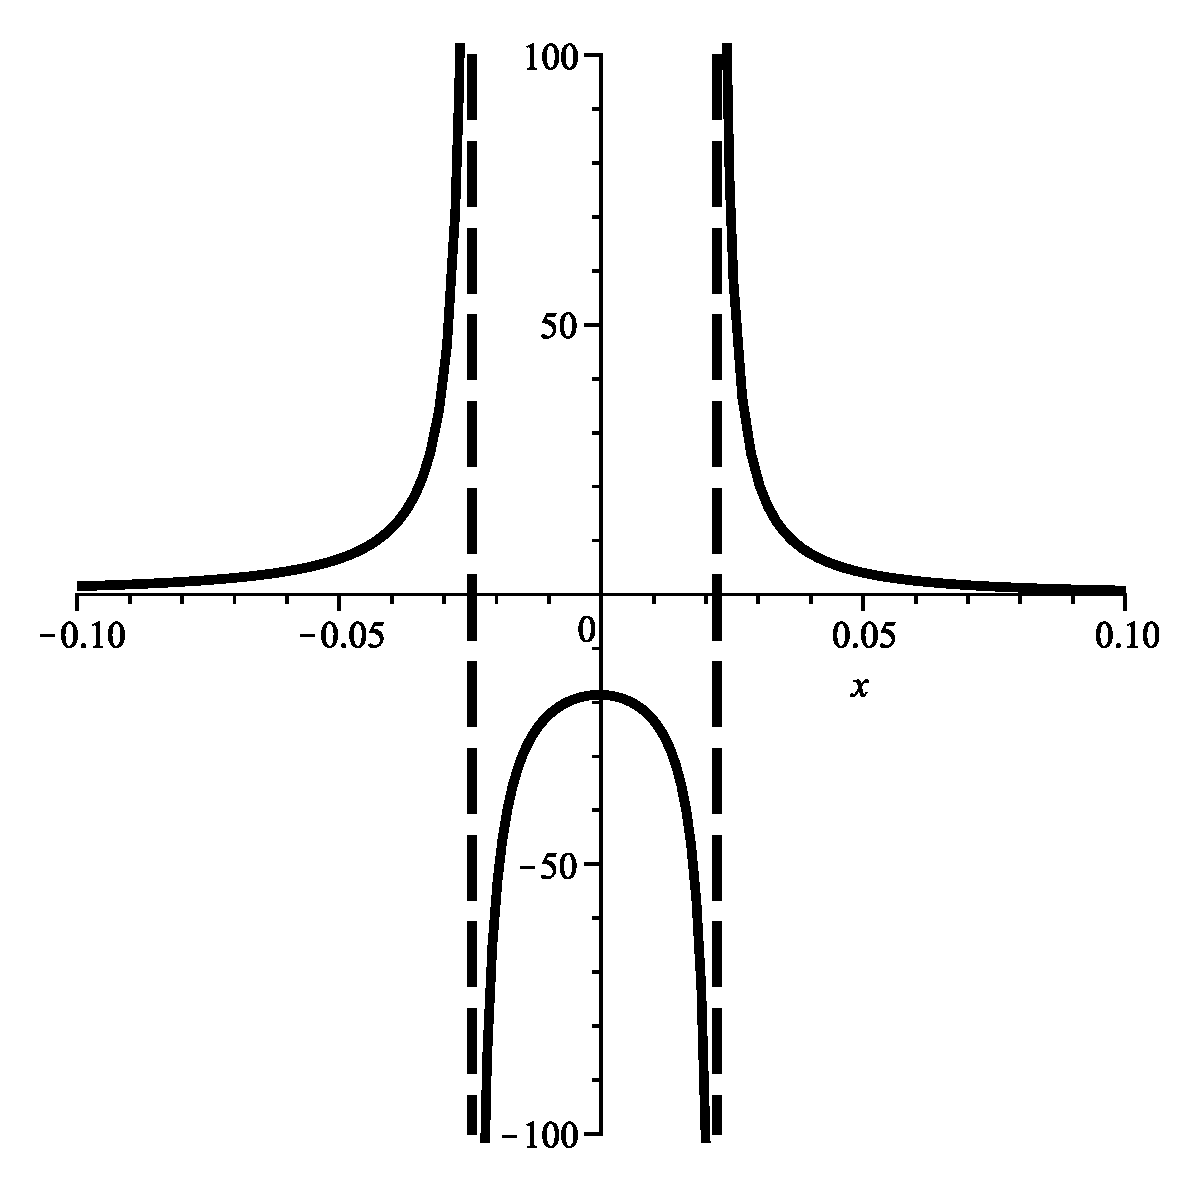
\includegraphics[scale=0.2]{figures/Picture.eps}}
\caption{This is the caption for the figure.}
\label{fig:Pict}
\end{figure}


\begin{figure}[!ht]
\centering
\missingfigure{If you know there will be a figure, but you still need to create it.}
\caption{This is the caption for the figure which is not even present.}
\label{fig:PictMis}
\end{figure}


Lorem ipsum dolor sit amet, consetetur sadipscing elitr, sed diam nonumy eirmod tempor invidunt ut labore et dolore magna aliquyam erat, sed diam voluptua. At vero eos et accusam et justo duo dolores et ea rebum. Stet clita kasd gubergren, no sea takimata sanctus est Lorem ipsum dolor sit amet. Lorem ipsum dolor sit amet, consetetur sadipscing elitr, sed diam nonumy eirmod tempor invidunt ut labore et dolore magna aliquyam erat, sed diam voluptua. At vero eos et accusam et justo duo dolores et ea rebum. Stet clita kasd gubergren, no sea takimata sanctus est Lorem ipsum dolor sit amet.\todo{This is a small Todo, please take care!}

or two side-by-side pictures:

\begin{figure}[!ht]
\centering
\subfigure{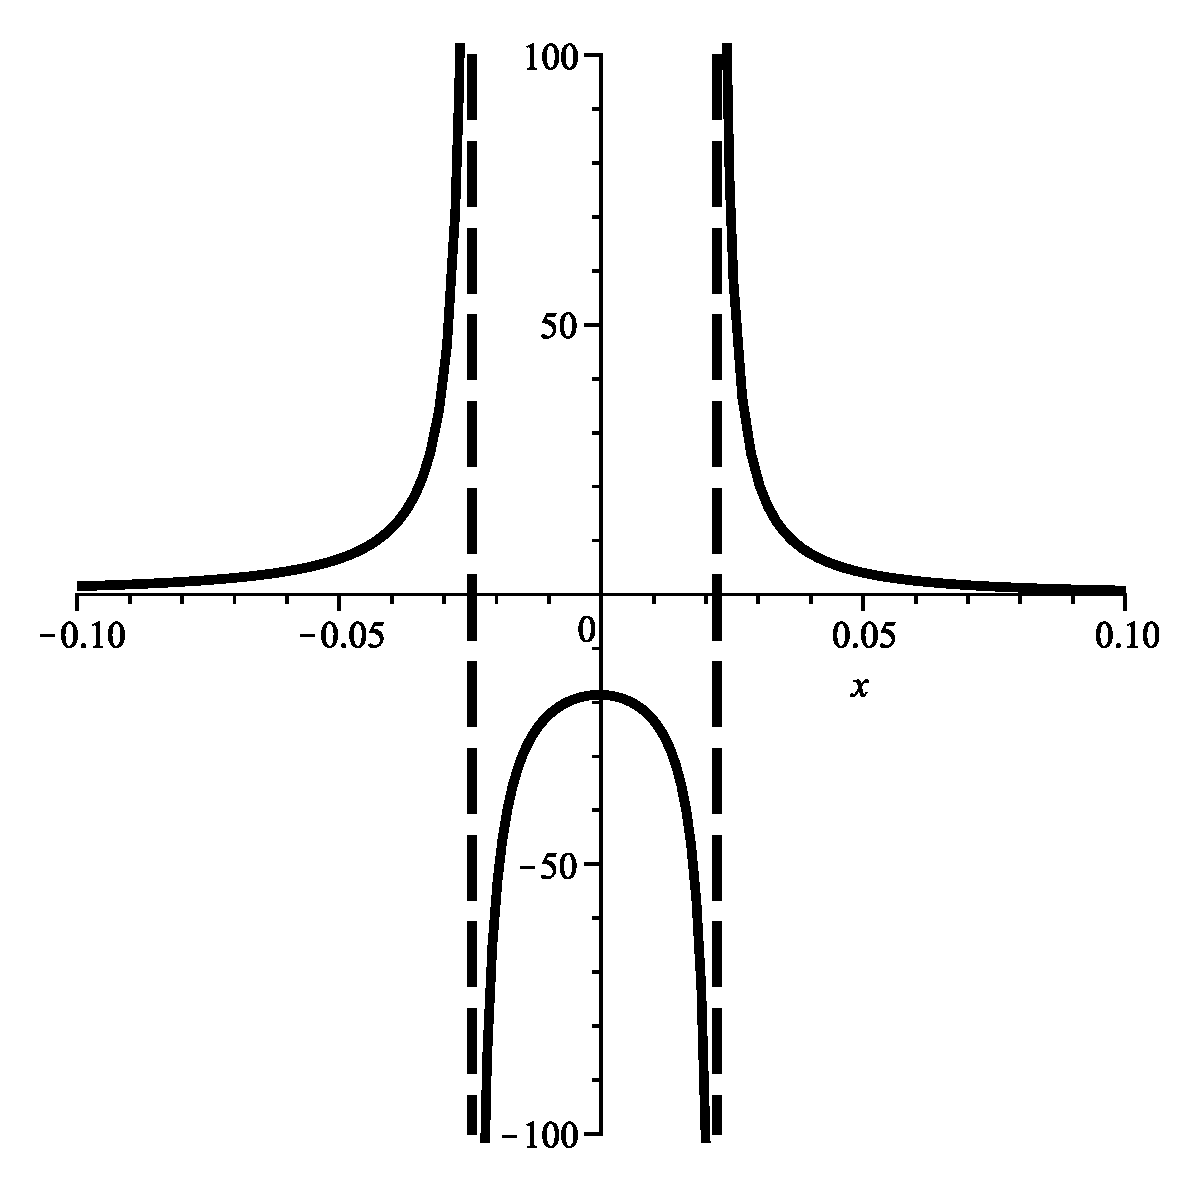
\includegraphics[scale=0.3]{figures/Picture.eps}}
\hspace{15pt}
\subfigure{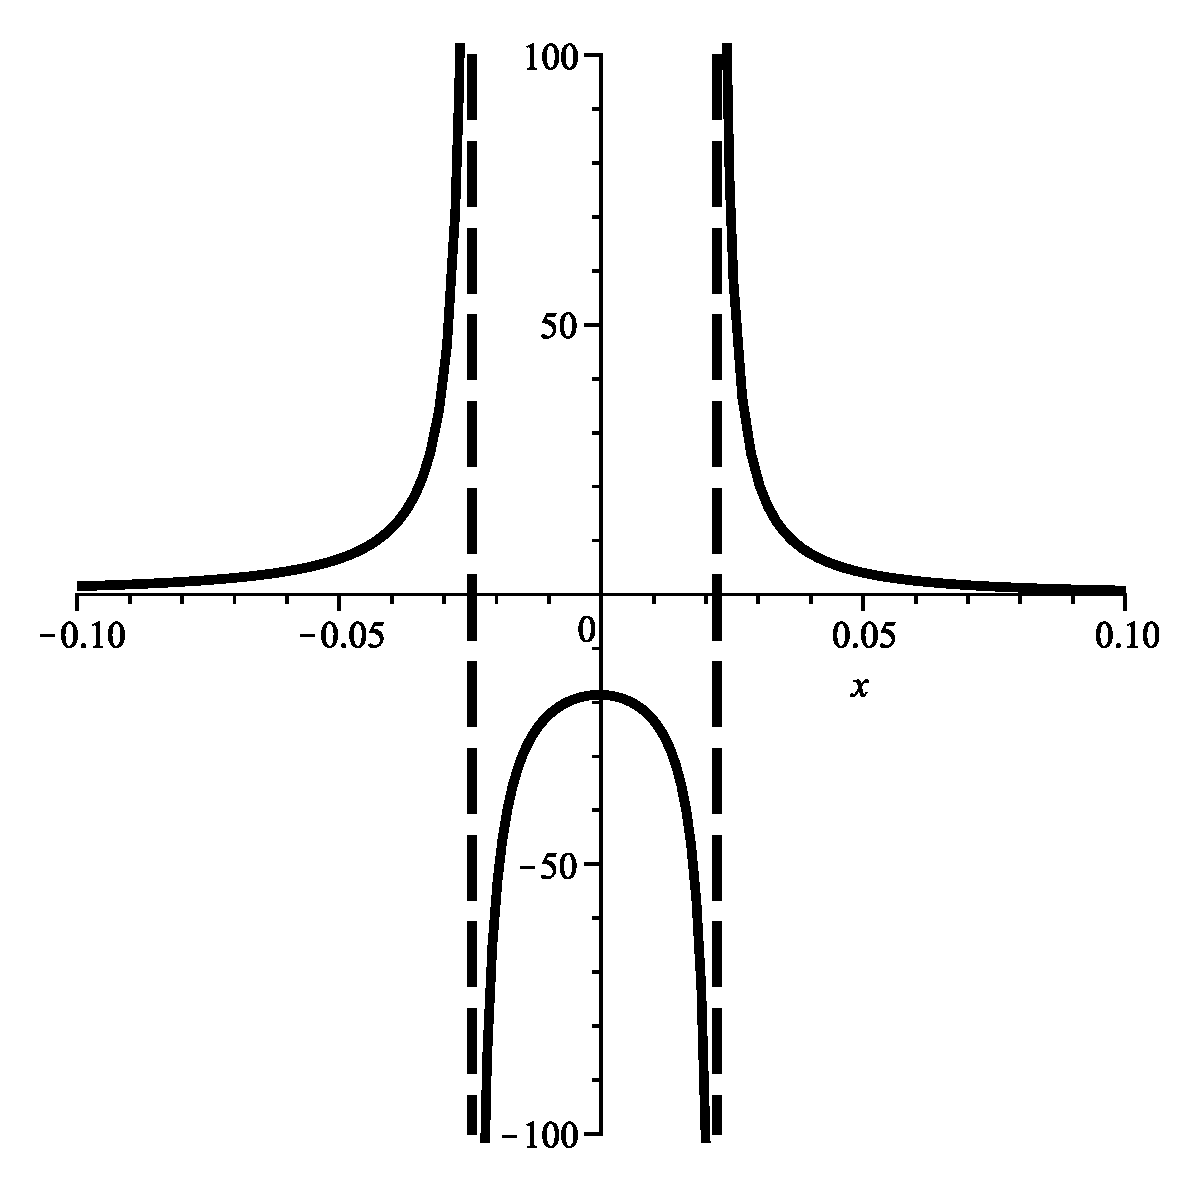
\includegraphics[scale=0.3]{figures/Picture.eps}}

\caption{Another caption}
\label{fig:Pict2}
\end{figure}



\subsection{Table}
Lorem ipsum dolor sit amet, consetetur sadipscing elitr, sed diam nonumy eirmod tempor invidunt ut labore et dolore magna aliquyam erat, sed diam voluptua. At vero eos et accusam et justo duo dolores et ea rebum. Stet clita kasd gubergren, no sea takimata sanctus est Lorem ipsum dolor sit amet. Lorem ipsum dolor sit amet, consetetur sadipscing elitr, sed diam nonumy eirmod tempor invidunt ut labore et dolore magna aliquyam erat, sed diam voluptua. At vero eos et accusam et justo duo dolores et ea rebum. Stet clita kasd gubergren, no sea takimata sanctus est Lorem ipsum dolor sit amet\explainindetail{This needs further explanation}.
\begin{table}[!ht]
	\centering
	\begin{tabular}{|l|rl|}
		\hline
		Something & Someother & Thing \\
  		Seems & to be & good\\
  		\hline
  	\end{tabular}
  	\caption{Random data for a table.}
\end{table}

Lorem ipsum dolor sit amet, consetetur sadipscing elitr, sed diam nonumy eirmod tempor invidunt ut labore et dolore magna aliquyam erat, sed diam voluptua. At vero eos et accusam et justo duo dolores et ea rebum. Stet clita kasd gubergren, no sea takimata sanctus est Lorem ipsum dolor sit amet. Lorem ipsum dolor sit amet, consetetur sadipscing elitr, sed diam nonumy eirmod tempor invidunt ut labore et dolore magna aliquyam erat, sed diam voluptua. At vero eos et accusam et justo duo dolores et ea rebum. Stet clita kasd gubergren, no sea takimata sanctus est Lorem ipsum dolor sit amet.


\section{Model calibration}
\subsection{What is calibration?}
Here is an example of a matrix\cite{website:fermentas-lambda} in $A\in\mathcal{M}_n(\RR)$:
$$
A = 
\begin{pmatrix}
a_{11} & a_{12} & \ldots & a_{1n}\\
a_{21} & \ddots & \ddots  & \vdots\\
\vdots &  \ddots & \ddots  & \vdots\\
a_{n1} &  \ldots &  \ldots & a_{1n}.
\end{pmatrix}
$$

\subsection{Numerical methods for calibration}
...



\section{Conclusion}
 It is a chapter to sum up the main points of the work, such as the aims and objectives of the project, the contributions and results you have achieved.  Future plan and development can be mentioned in this section.

\newpage
%\nomenclature{$a$}{The number of angels per unit area}%
%\nomenclature{$N$}{The number of angels per needle point}%
%\nomenclature{$A$}{The area of the needle point}%
%\printnomenclature


\newacronym{lvm}{LVM}{Logical Volume Manager}
\newglossaryentry{pi}
{
  name={\ensuremath{\pi}},
  description={ratio of circumference of circle to its
               diameter},
  sort=pi
}
\newglossaryentry{Linux}
{
  name=Linux,
  description={is a generic term referring to the family of Unix-like
               computer operating systems that use the Linux kernel},
  plural=Linuces
}
\printglossaries

\newpage
%%%%% References
\bibliographystyle{ieeetr}
\bibliography{bibs/sample1, bibs/sample2} 
%%%%% Declaration
%\thispagestyle{empty}


\mbox{}\newline\vspace{10mm} \mbox{}\LARGE
%
{\bf Declaration} \normalsize \vspace{5mm}

I declare that this thesis is the solely effort of the author.
I did not use any other sources and references than the listed ones. I have marked all contained direct or indirect statements from other sources as such.

Neither this work nor significant parts of it were part of another review process.
I did not publish this work partially or completely yet.
The electronic copy is consistent with all submitted copies.

\bigskip
\bigskip
\bigskip
\bigskip


Signature and date: 






%%%%% Appendix 
\appendix

\section{Review of stochastic calculus}
\subsection{Riemann integration}
\subsection{The It\^o integral}



%%%%%%%%%%%%%%%%%%%%%%%%%%%%%%%%%%%%%%%%%%%%%%%%%%%%
%%%%%%%%%%%%%%%%%%%%%%%%%%%%%%%%%%%%%%%%%%%%%%%%%%%%
%%%%%%%%%%%%%%%%%%%%%%%%%%%%%%%%%%%%%%%%%%%%%%%%%%%%
%%%%%%%%%%%%%%%%%%%%%%%%%%%%%%%%%%%%%%%%%%%%%%%%%%%%


\end{document}
